%%%%%%%%%
\begin{figure*}
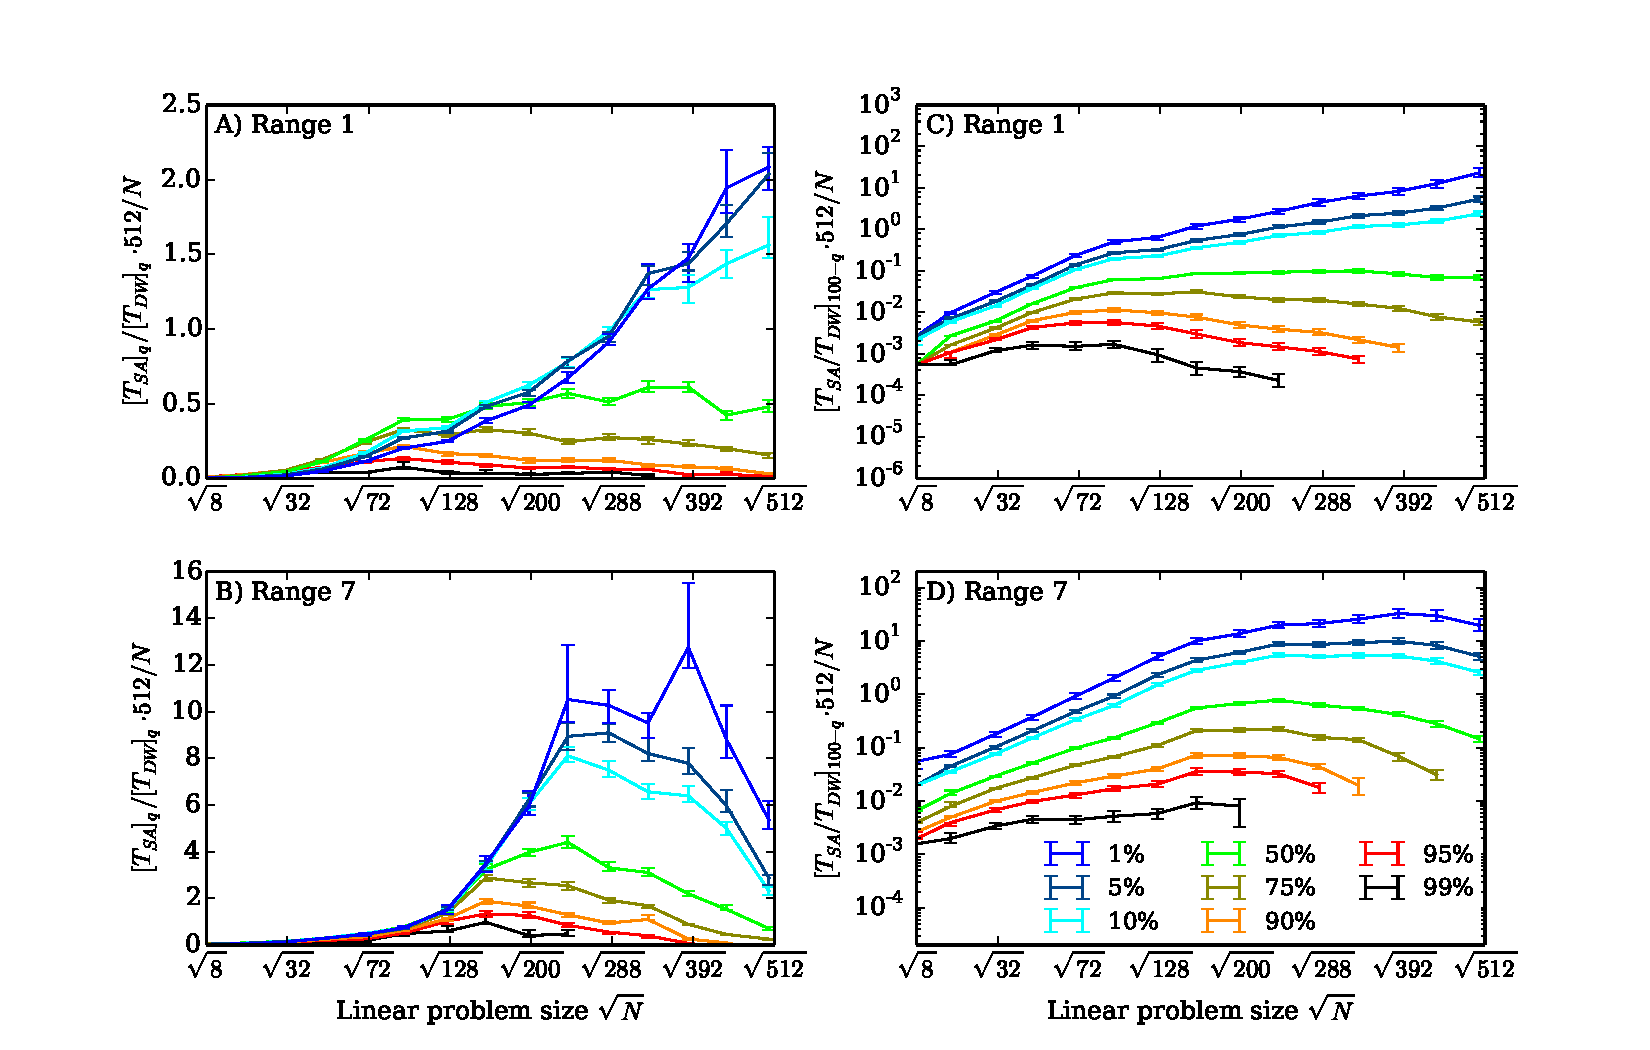
\includegraphics[width=0.95\textwidth]{fig07.pdf}
\caption{{\bf Speedup of the DW2 compared to SA.} A) and B) for the ratio of the quantiles (RofQ), C) and D) for the quantiles of the ratio (QofR). For a random variable $X$ with distribution $p(x)$ and values in $x\in [0,\infty)$ we define, as usual, the $q$th quantile as $\int_0^{x_q} p(x) dx = q/100$, which we solve for $x_q$ and plot as a function of $\sqrt{N}$. In the QofR case we use $x_{100-q}$  so that high quantiles still correspond to instances that are hard for the DW2. We terminate the curves when the DW2 does not find the ground state for large $N$ at high percentiles. In these plots we multiplied Eqs.~\eqref{eq:S_q} and \eqref{eq:SQoR} by $512$ so that the speedup value at $N=512$ directly compares one DW2 processor against one classical CPU. An overall positive slope suggests a possible limited quantum speedup, subject to the caveats discussed in the text. A negative slope indicates that SA outperforms the DW2.
}
\label{fig:qorspeedup7}
\end{figure*}
%%%%%%%%%
